\documentclass[a4paper, 11pt, oneside]{article}
\usepackage[svgnames]{xcolor}
\usepackage{graphicx} % Required for box manipulation
\usepackage{geometry}
\usepackage{pgfplots}
\pgfplotsset{compat=1.14}
\geometry{legalpaper, margin=1in}
\newcommand*{\plogo}{\fbox{$\mathcal{PL}$}} % Generic dummy publisher logo

\usepackage[utf8]{inputenc} % Required for inputting international characters
\usepackage[T1]{fontenc} % Output font encoding for international characters
\usepackage{PTSerif} % Use the Paratype Serif font
\usepackage{amsmath}
\usepackage{amssymb}
\usepackage{chngcntr}
\counterwithin*{subsection}{section}
\usepackage{graphicx}
\graphicspath{}

\begin{document}

\begin{center}  % Centre all text
	
	%------------------------------------------------
	%	Title and subtitle
	%------------------------------------------------
	
	\setlength{\unitlength}{0.6\textwidth} % Set the width of the curly brackets above and below the titles
	
	{\color{LightGoldenrod}\resizebox*{\unitlength}{\baselineskip}{\rotatebox{90}{$\}$}}}\\[\baselineskip] % Top curly bracket
	
	\textcolor{Sienna}{\textit{\Huge MAST90045\\ $\;$ \\Systems Modelling and Simulation}}\\[\baselineskip] % Title
	
	{\color{RosyBrown}\Large Assignment 3}\\ % Subtitle or further description
	
	{\color{LightGoldenrod}\resizebox*{\unitlength}{\baselineskip}{\rotatebox{-90}{$\}$}}} % Bottom curly bracket
	
	 % Whitespace between the title and the author name
	
	%------------------------------------------------
	%	Author
	%------------------------------------------------
	
	{\Large\textbf{Chris Swan 370502}}\\ % Author name
	
	
	
	%------------------------------------------------
	%	Publisher
	%------------------------------------------------
	
	%\plogo\\[0.5\baselineskip] % Publisher logo
	
	University of Melbourne % Publisher name

\end{center}

\tableofcontents


\section{Problem Introduction: Conserving Water}

As the world turns toward modernity, water conservation becomes a more critical.  Whilst populations may plateau in developed contries, the water consumption of of these nations is significant per capita, with a household using water for washing clothes, showering, drinking, gardening, cooking; it is intrinsically bound up in our daily lives.  Therefore being able to simmulate how water might be saved, even just as a general approximation, is a powerful tool indeed.  \\

Our study here concerns how installing rainwater and greywater tanks for a home and using this water for activities such as flushing the toilet and watering the garden might help to minimise a home's water consumption.  Doing this for just these basic activities can, as we shall demonstrate, have a significant impact on water reduction, and offer a baseline for extrapolation as to what other activities might recycled water be made use of.

\section{Task 1: Simmulating Monthly Rainfall}

We have at our disposal average monthly rainfall data of Melbourne for approximately 100 years.  Before making use of this however, we must begin by finding some means of simmulating rain; that is, a statistical method of predicting whether or not it will rain and a method of determining how much rain will fall.  We expect the probability of rainfall per day to be low - perhaps $0.2$, although this is hard to say given we're simulating Melbourne weather!  Additionally, across a month, we would expect the most total depths of rainfall to be between 0 and 40, with the frequency decreasing significantly soon after this.\\

Letting $X_{i,j}$ be the rainfall of the $j^{\text{th}}$ day of the $i^{\text{th}}$ month, we have the following assumptions:

\begin{flalign*}
X_{i,j} &\sim A_{i,j} B_{i,j}, \; \text{ for } A_{i,j} \text{ and } B_{i,j} \text{ independent, with } \\
A_{i,j} &\sim Bernoulli(p_i) \\
B_{i,j} &\sim Gamma(m_i, \lambda_i)
\end{flalign*}

We assume for the sake of simplicity that the probability of rainfall from one to day to the next are independent events, though we know in reality this is not the case.  Nonetheless, this will still provide some picture of rainfall at least.  \\


We define two functions to simulate this: one to model the depth of water for a given month ($Y_{sim}$) and another to model the cummulative probability density for the likelihood of rainfall ($F_Y$).\\

For $n_i$ being the number of days in month $i$, we have the rainfall for that month as $$Y_i = \sum_{j=1}^{n_i} X_{i,j}$$

From this this and our earlier assumptions, we can infer the following for our function $Y_{sim}$:

\begin{flalign*}
\text{For some month } i:\\
\mathbb{E}(A) &= p\\
\mathbb{E}(B) &= \frac{m}{\lambda}\\
\mathbb{E}(X) &= \mathbb{E}(A \cdot B)\\
\text{Given } A \text{ and } B \text{ being independent:}\\
\mathbb{E}(X) &= \mathbb{E}(A) \cdot \mathbb{E}(B)\\
\therefore X &= \frac{p \cdot m}{\lambda}\\
\text{We further have that: }\\
\mathbb{E}(Y) &= \mathbb{E}(\sum_{j=1}^n X) \text{ (Assuming i.i.d.)}\\
\mathbb{E}(Y) &= \sum_{j=1}^n \mathbb{E}( X)\\
\mathbb{E}(Y) &= \sum_{j=1}^n \frac{p \cdot m}{\lambda}\\
\therefore \mathbb{E}(Y) &= \frac{n \cdot p \cdot m}{\lambda}
\end{flalign*}


Similarly, for our function $F_Y$, we have that:

\begin{flalign*}
\text{For some month } i:\\
\text{Let } N &= \sum_{j=1}^n A_{j} \sim binom(n, p) \\
\text{For } x \geq 0:\\
Pr(Y \leq x) &= Pr(N = 0) + \sum_{k=1}^n Pr(\Gamma(k \cdot m, \lambda) \leq x) Pr(N=k)\\
\end{flalign*}

We will attempt to better explain how this is achieved with words rather than notation.\\

$ \sum_{k=1}^n Pr(\Gamma(k \cdot m, \lambda) \leq x) Pr(N=k)$ represents the total rainfall for the month up to $x$ (see Figure 1).  $\Gamma(k \cdot m, \lambda)$ generates rainfall for a day of the month, so summing across $n$ gives a month of rainfall, with $binom(n,p)$ generating a binary value determining whether or not it will rain on that day. (As our Gamma random variables are independent, the sum of $\Gamma(m_1, \lambda)$ and $\Gamma(m_2, \lambda)$  has a $\Gamma(m_1 + m_2, \lambda)$ distribution.)\\

$Pr(N = 0)$ will thus return the probability that it does not rain on any day in the month and $Pr(N = k)$ will return the probability that it rains on $k$ days.  These elements bound together in the function $Pr(Y \leq x) = Pr(N = 0) + \sum_{k=1}^n Pr(\Gamma(k \cdot m, \lambda) \leq x) Pr(N=k)$ will return a cummulative density function for the month.\\

\begin{figure}[h]
\centering
\caption{\textbf{Cummulative density function ($F_Y$).}  The likelihood of that in any month it will rain less than a depth of $x$}
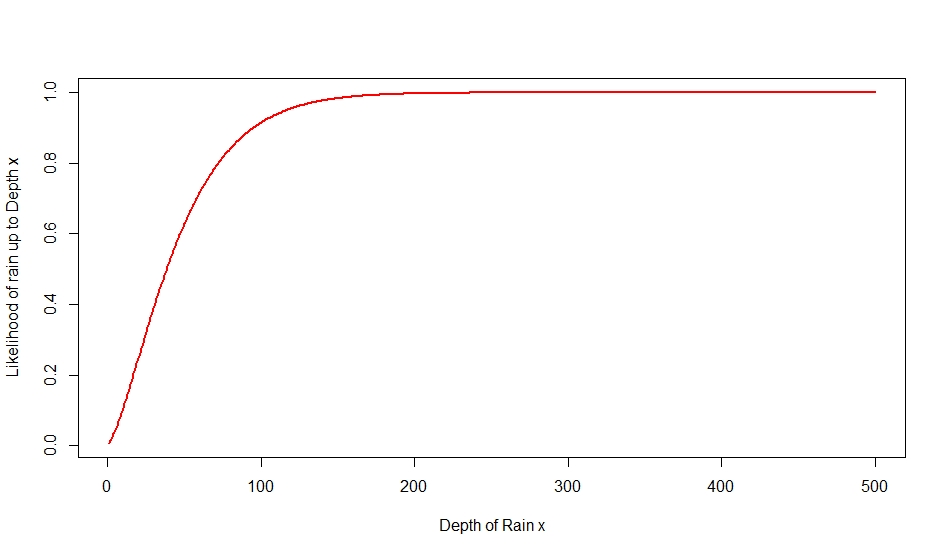
\includegraphics[width = \textwidth]{CDF}
\end{figure}

We next use to Ysim to generate $10^4$ instances of rainfall from some default parameters ($p=0.27$, $m=0.24$, $\lambda = 0.043$) and store these in a vector.  We then feed this vector into $F_Y$ and generate a cummulative density plot of the likelihood of a depth of rain for any month; that is, the probability that it will not rain \emph{more} than the value in the x axis (see Figure 1).\\

From this we develop a means of simulating rainfall for a certain day and extending this across the months of a year.  We can then estimate our paramaters need for create a simmulation of average rainfall and thereby simmulate the water usage of a home.\\

Finally, we plot the simulated values of $Y_{sim}$ and compare the observed values for each bin with the expected value given by $F_Y$ (see Figure 2).  This gives us a good idea of the accuracy of our functions and their applicability for estimating parameters in Part 2.\\

\begin{figure}[h]
\centering
\caption{\textbf{Plot of $Y_{sim}$ for $10^4$ month simulations.} The first bin indicates days in which rainfall was of a depth between 0 and 20, the second between 20 and 40, etc.  Blue points are the mean depth of rain within each bin from $F_Y$ and redl lines are similarly the condifence intervals obtained from $F_Y$.}
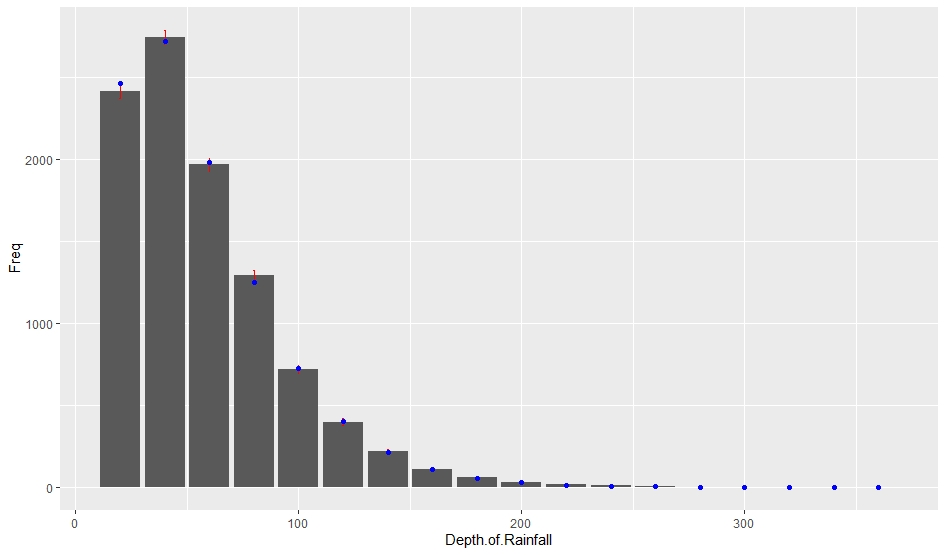
\includegraphics[width = \textwidth]{BinFreq}
\end{figure}

\newpage
\section{Task 2: Estimating Parameters}

In estimating the parameters for our upcoming simulation, we use the Melbourne rainfall data.  We expect these parameters to estimate those needed for our simulation reasonably well, given the large corpus and period the data is averaged over.  We import each columns of the dataframe as a vector and so obtain values for each month.  \\

$\hat{p}_i$ is obtrain directly from the dataframe, from the feature (column) "mean\_days\_rain".\\

$\hat{m}_i$ can be found from rearranging the formula of $\mathbb{E}(Y_i)$ that we found above, which gives us:

$$\hat{m}_i = \frac{\hat{y}_i \cdot \hat{\lambda}_i}{dm_i \cdot \hat{p}_i}$$

where $dm$ are the number of days in month $i$ and $\hat{y}_i $ is from the feature "mean\_rainfall" in the dataframe.  This leaves $\hat{\lambda}_i$ as our unknown parameter, which we find with the following loss function:






\section{Summary}





\newpage

\section{Appendices}

\subsection{A: Code}

\begin{verbatim}

rm(list=ls())

# Part 1


dm = c(31,28,31,30,31,30,31,31,30,31,30,31) # days in a month

# testing distributions in R

set.seed(13)

rbinom(n = 31, size = 1, prob = 0.27)*rgamma(31,0.24,0.043)


# Ysim function

Ysim = function(p, m, la, n) {
  
  A = rbinom(n = n, size = 1, prob = p)
  
  B = rgamma(n = n, shape = m, rate = la)
  
  return(sum(A*B))

}



# F_Y function - we need to use dbinom, NOT pbinom!

F_Y = function(x, p, m, la, n) {
  my_list = c()
  for(k in 1:n) {my_list = 
    append(my_list, 
           pgamma(x, shape = k*m, rate = la)*dbinom(k, size = n, p))}
  
  cd_Y = dbinom(0, n, p) + sum(my_list)
  return(cd_Y)
}


# CDF of F_Y

xs = 1:500

fYplt = c()
set.seed(13)
for(a in 1:length(xs)) fYplt = append(fYplt, F_Y(a, 0.27, 0.24, 0.043, 31))

plot(x = xs, y = fYplt, type = 'l', col = 'red', lwd = 2, xlab = 'Depth of Rain x',
     ylab = 'Likelihood of rain up to Depth x')



# Import rain data

data = read.csv(file = "D:/School/Mast of Sci/MAST90045/A3/Melbourne_rainfall_mm-1.csv")


# Using Ysim to check F_Y is correct
set.seed(13)
Ysim(0.27,0.24,0.043,31)

# checking this will work...
lh = c(rep(NA,10^4))
for(k in 1:10^4) lh[k] = Ysim(0.27,0.24,0.043,31)

max(lh)


# making our bins
binsize = c(seq(0,360,20))

Bins = findInterval(lh, binsize)
Bins2 = as.data.frame(table(Bins))

Bins2


mod_fY = function(x) return(F_Y(x, 0.27,0.24,0.043,31))

set.seed(13)
(mod_fY(20) - mod_fY(0))*10^4

#Standard deviation
sqrt((mod_fY(20) - mod_fY(0))*10^4*(1- mod_fY(20) + mod_fY(0)))

# Generate the frequencies
Fmean = c()
Fsd = c()
for(i in c(seq(0,340,20))) {
  Fmean = append(Fmean, (mod_fY(i+20) - mod_fY(i))*10^4)
  Fsd = append(Fsd, sqrt((mod_fY(i + 20) - 
                            mod_fY(i))*10^4*(1- mod_fY(i + 20) + mod_fY(i))))
}

freq = Bins2$Freq
FRE = c(freq[1:14],0,0,freq[15:16])
FRE

#Getting everything into a nice dataframe for plotting
BINS = data.frame('Depth of Rainfall' = seq(20,360,20), 
                  'Freq' = FRE, 'Mean' = Fmean, 'SD' = Fsd )
BINS




library(ggplot2)

H = ggplot(BINS, aes(Depth.of.Rainfall, Freq), ) + geom_bar(stat = 'identity') +
  geom_errorbar(aes(ymin = Freq-SD, ymax = Freq+SD), width =.5, colour = 'red') +
  geom_point(aes(y=Mean), colour = 'blue')
  

print(H)


# Part 2

#defining parameters
p_est = c()
x_est = c()
dec_1 = c()
dec_5 = c()
dec_9 = c()
y_est = c()
for(i in 1:12) {
  p_est = append(p_est, data$mean_days_rain[i]/dm[i])
  x_est = append(x_est, data$mean_rainfall[i]/dm[i])
  dec_1 = append(dec_1, data$decile_1_rainfall[i])
  dec_5 = append(dec_5, data$median_rainfall[i])
  dec_9 = append(dec_9, data$decile_9_rainfall[i])
  y_est = append(y_est, data$mean_rainfall[i])
}

# lambda function test?

L = function(lambda) {
  jingo = (100/9)*(F_Y(x = dec_1[1], 
                       p = p_est[1], 
                       m =( y_est[1]*lambda)/(dm[1]*p_est[1]), 
                       la = lambda, n = dm[1] )-0.1)^2 + 
    4*(F_Y(x = dec_5[1], 
           p = p_est[1], 
           m =( y_est[1]*lambda)/(dm[1]*p_est[1]), 
           la = lambda, n = dm[1] )- 0.5)^2 + 
    (100/9)*(F_Y(x = dec_9[1], 
                 p = p_est[1], 
                 m =( y_est[1]*lambda)/(dm[1]*p_est[1]), 
                 la = lambda, 
                 n = dm[1] )-0.9)^2
  return(jingo)
}

#testing optimsation
optim(par = 0.5, fn = L)$par

# actual lambda function

L = function(lambda) {
  jingo = (100/9)*(F_Y(x = dec_1[i], 
                       p = p_est[i], 
                       m =( y_est[i]*lambda)/(dm[i]*p_est[i]), 
                       la = lambda, 
                       n = dm[i] )-0.1)^2 + 
    4*(F_Y(x = dec_5[i], 
           p = p_est[i], 
           m =( y_est[i]*lambda)/(dm[i]*p_est[i]), 
           la = lambda, n = dm[i] )- 0.5)^2 + 
    (100/9)*(F_Y(x = dec_9[i], 
                 p = p_est[i], 
                 m =( y_est[i]*lambda)/(dm[i]*p_est[i]), 
                 la = lambda, 
                 n = dm[i] )-0.9)^2
  return(jingo)
}

lam_est = c()
lam_sd = c(rep(NA,12))
for(i in 1:12) {
  lam_est = append(lam_est, optim(par = 0.5, fn = L)$par)
  lam_sd[i] = optim(par = 0.5, fn = L)$value
}

m_est = c(rep(NA,12))
for(i in 1:12) m_est[i] = (y_est[i]*lam_est[i])/(dm[i]*p_est[i])

print(lam_est)
print(m_est)
print(p_est)


library(stats)
sd(lam_est)
sd(p_est)
sd(m_est)


# Part 3 


month = function(day){
  dys = c(31,59,90,120,151,181,212,243,273,304,334,365)
  m = c(1:12)
  for (i in 1:length(dys)) {
    if (day <= dys[i]) {
      return(m[i])
    }
  }
}

tanksim = function(num_years, maxraintank, maxgreytank, 
                   phat = p_est, mhat = m_est, lahat = lam_est, plotflag = F) {
  # Constants
  days = 1:365
  days_in_month = c(31, 28, 31, 30, 31, 30, 31, 31, 30, 31, 30, 31)
  mean_max_temp = c(25.9, 25.8, 23.9, 20.3, 16.7, 14.1, 13.5, 15.0, 
                    17.2, 19.7, 22.0, 24.2)
  roofarea = 100 # m^2
  gardenarea = 200 # m^2
  flushsize = 5 # litres per flush
  numflush = function() rbinom(1, 15, .8) # flushes per day 
                                          #for four people, at home half the day
  showersize = 35 # in litres
  numshower = 4 # showers per day for four people
  washsize = 35 # litres per load
  numwash = function() rbinom(1, 8, .125) # washes per day for four people
  
  Xsim = function(month) {
    # simulate rainfall for a day in given month
    rbinom(1, 1, phat[month])*rgamma(1, mhat[month], lahat[month])
  }
  
  save_year = c(rep(NA, length(num_years)))
  tank_rain_av = c(rep(0, 365))
  grey_rain_av = c(rep(0, 365))
  yearly_raintank = matrix(NA, nrow = 365, ncol = num_years)
  yearly_greytank = matrix(NA, nrow = 365, ncol = num_years)
  
  
  for (year in 1:num_years) {
    raintank = c(rep(0, 365))
    greytank = c(rep(0, 365))
    daily_saved = c(rep(0, 365))
    gardenwater = c(rep(0, 365))
    for (i in 1:365) {
      M = month(i) 
      rain = Xsim(M) 
      flushwater = numflush() * flushsize
      
      raintank[i] =  raintank[i] + (roofarea * rain)
      greytank[i] = greytank[i] + (numshower * showersize) +
        (numwash() * washsize)
      if (raintank[i] > maxraintank) raintank[i] = maxraintank
      if (greytank[i] > maxgreytank) greytank[i] = maxgreytank
      
      avMAXtemp = mean_max_temp[M]/15
      gardenwater[i] = rain*gardenarea
      if (i < 3) avggardenwater = sum(gardenwater[1:i])/i
      else avggardenwater = mean(gardenwater[(i-2):i])
      
      if (flushwater <= greytank[i]) greytank[i] = greytank[i] - flushwater
      else if (flushwater <= (raintank[i] + greytank[i])) {
        raintank[i] = raintank[i] + greytank[i] - flushwater
        greytank[i] = 0
      } 
      else {
        greytank[i] = 0
        raintank[i] = 0
      }
      
      if (avggardenwater < avMAXtemp) gardenreq = avMAXtemp - avggardenwater 
      else gardenreq = 0
      
      if (gardenreq*gardenarea <= raintank[i]) {raintank[i] = raintank[i] - 
        gardenarea*gardenreq}
      else if (gardenreq*gardenarea <= (raintank[i] + greytank[i])) {
        greytank[i] = greytank[i] + raintank[i] - gardenreq*gardenarea
        raintank[i] = 0
      } 
      else {
        greytank[i] = 0
        raintank[i] = 0
      }
      daily_saved[i] = raintank[i] + greytank[i]
      if (i < 365){
        raintank[i+1] = raintank[i]
        greytank[i+1] = greytank[i]
      }
    }
    save_year[year] = sum(daily_saved)
    yearly_greytank[,year] = greytank
    yearly_raintank[,year] = raintank
  }
  total_grey = c()
  total_rain = c()
  for (n in 1:num_years) {
    
    total_grey = c(total_grey,yearly_greytank[,n])
    total_rain = c(total_rain, yearly_raintank[,n])
    
  }
  
  if (plotflag == T) {

    plot(x = 1:length(total_rain), y = total_rain,
         type = "l", col = "blue", xlab = "Days", ylab = "Litres",
         lwd = 0.5)
    lines(x = 1:length(total_grey), y = total_grey,
          type = "l", col = "red", lwd = 0.5 )
    }
  total_save = sum(save_year)
  return(total_save)
}


tanksim(5, 3000, 1000, p_est, m_est, lam_est, T)


#prelim exploration of most water saved for different tank sizes for a 5 year period

I = c(seq(2000,10000,500))
J = c(seq(500,8500,500))
B = 0
for (i in I) {
  for (j in J) {
    A = tanksim(5,i,j,p_est, m_est,lam_est,F)
    if (A > B) {
      B = A
      best_i = i
      best_j = j
    }
  }
}
cat('Best Rainwater Tank Size: ', best_i, '\n Best Greywater Tank Size: ', best_j,
    '\n Water Saved: ', B)
tanksim(5,10000,8000,plotflag = T)

tanksim(10,10000,8000,plotflag = T)


I = c(seq(2000,50000,500))
J = c(seq(500,48500,500))
B = 0
for (i in I) {
  for (j in J) {
    A = tanksim(10,i,j)
    if (A > B) {
      B = A
      best_i = i
      best_j = j
    }
  }
}
cat('Best Rainwater Tank Size: ', best_i, '\n Best Greywater Tank Size: ', best_j,
    '\n Water Saved: ', B)

tanksim(10,best_i, best_j, plotflag = T)

\end{verbatim}




\end{document}
